% Anurag and 
% Akshay to PR - COMPLETED 1

\chapter{Project Planning \& Management} \label{Chapter:Project Planning & Management}


\section{Team Management}
In this section, the document discusses the team management and the planning made throughout the project in order to successfully reached the aims set in the project specification.

\subsection{Project Management Plan and Technique}
Prior to the start-up of the project, the team had a meeting to introduce and get to know each other, before assigning the role of Project Manager and Vice President (VP) of Assessment. As the discussion goes on, the project was broken down into the main components, known as a Work Breakdown Structure (WBS), which turned the overwhelming work loads into manageable pieces. An individual skills assessment has been created within the team so that the components can be divided to each of the member depending on their ability, knowledge and the comfortability to handle the task. This is discussed later in the Division of Responsibility Section \ref{section: division of responsibility}. Together, with the official deadlines released by the University, a Gantt chart, which is a visual timeline across the life cycle of a project is made, with start and estimated end dates for each of the individual tasks set up. The Gantt Chart is discussed further in Section \ref{gantt_chart}. Throughout the project, the Gantt Chart was regularly modified and updated to include more detailed tasks as a subsection of the main components. Using the Gantt chart, the scheduled work loads that were planned initially can be compared with the actual timelines of the project, keeping on track for our goals and final deliverables.
                                                                  
A Kanban management method \cite{landau_2019} is used for this project, using a collaboration tool Trello to organize and keeping track, where any small tasks or deadline were recorded into boards, specifying person-in-charge, what is being worked on, and the progress. To further ensure the project remained on track, there were at most three meetings scheduled per week.
\begin{itemize}
    \item Monday – Unofficial meeting with the team members, mainly to discuss to progress made within the past week and preparation to make for the official meeting on Tuesday.
    \item Tuesday – Official meeting with external partner InterDigital to discuss the project progress and development.
    \item Thursday – Meeting with supervisor to update the progress made on respective week, and to discuss any matter about the project.
\end{itemize}

All the discussion, idea for development, progress and on-going tasks were kept in meeting minutes by the project manager. A list of tasks, based on a weekly sprint approach, where on-going, priority and completed tasks were set, as shown in Appendix \ref{fig:WBS1}. The length of time each task took the team member can be seen. Once the task was completed they would be assigned a new task. This was completed after the meeting and attached in an email thread that included all the team members, supervisor and our InterDigital partner. As the project goes on, hard internal deadlines were decided upon in order to motivate and push the team members. These were important especially as University deadlines for the Presentations to InterDigital, to the University and for the group report. 

\subsubsection{Presentation Planning}
For the several presentations made to the both InterDigital and to the University, the sections were split into the three stages as described in the system design as well as the overall system and project management. Each member would present the stage they were in charge of and time allotments were provided to each member. Editing to unify the slides and appropriate slide transitions were handled by the Project Manager. Slide assignments were given in order to ensure every member would speak for the same duration.

\subsubsection{Final Report}
A skeleton or content draft was made by VP of Assessments as a guide to assist the \textit{Group Report}. This is seen in Appendix \ref{appendix:report_planning} and shows how each team member was assigned an initial section to document the work. As the write-up developed, new sub-sections would be added if needed to the planning document. Before the write-up began, the team held a week long work session to develop technical aspects of the project, and then all focus switched to the write-up. 

Based on the involvement during the project, each of the team members were responsible to write their research, implementation, results and discussion on the part they were assigned to initially. Depending on the progress made, the remaining work was divided equally, taking into consideration the time availability of the person, ensuring everyone works fairly and at the same pace with the same workloads. Throughout the writing period, a daily meeting was held at the end of each day to keep track of everyone’s work and progress, as well as motivating each other for the last push of the project.

\subsection{Division of Responsibility}
\label{section: division of responsibility}
Below is the roles and responsibilities assigned to each of the members in order to get the project to progress smoothly. 

\textbf{Project Manager - }
Individual responsible to deliver the project by leading and managing project team on a day-to-day basis, communicating with each of the team members regarding the tasks assigned and checking the progress. Project manager also has an important role in interfacing between the team, supervisor and external partner from the respective company collaborated with. Specific responsibilities of project manager:
\begin{itemize}
    \item Set up the communication medium for the members to discuss the progression of tasks.
    \item Scheduling meetings between the team members, supervisor and external partner.
    \item Keeping the minute meetings.
    \item Summarize the discussion made during the meetings, next tasks assigned for each member for the record of supervisor and the external partner, through an email thread.
    \item Monitor overall progress of the project.
\end{itemize}

\textbf{Vice President (VP) of Assessment - }
A role where the person in charge needs to review the criteria needed in the assessment, remind the deadlines of each submission and responsible as a representative from the team to do the submissions.

\textbf{Project Team Members - }
Under the supervision and direction of the project manager, the team members are responsible for carrying out work detailed in the project plan. The project can be broken down into 5 main sections.

\begin{table}[ht]
\centering
\begin{tabular}{ |c|p{9cm}|c| } 
 \hline
 \textbf{Index} & \textbf{Main Task} & \textbf{Person-in-Charge}\\ 
  \hline
1 & Router Data Collection and Processing & Akshay \\ 
  \hline
2 & Edge Node Research, Implementation and Deployment & Syuhada, Anurag \\ 
  \hline
3 & Cloud Based Storage and Processing & Anurag \\ 
  \hline
4 & Cloud Based Processing and ML Development & Eu Jin \\ 
  \hline
5 & Create OTT application & All \\ 

 \hline
\end{tabular}
\caption{Task assignment and the person-in-charge. }
\label{table:task_management}
\end{table}

\begin{figure}[ht]
    \centering
    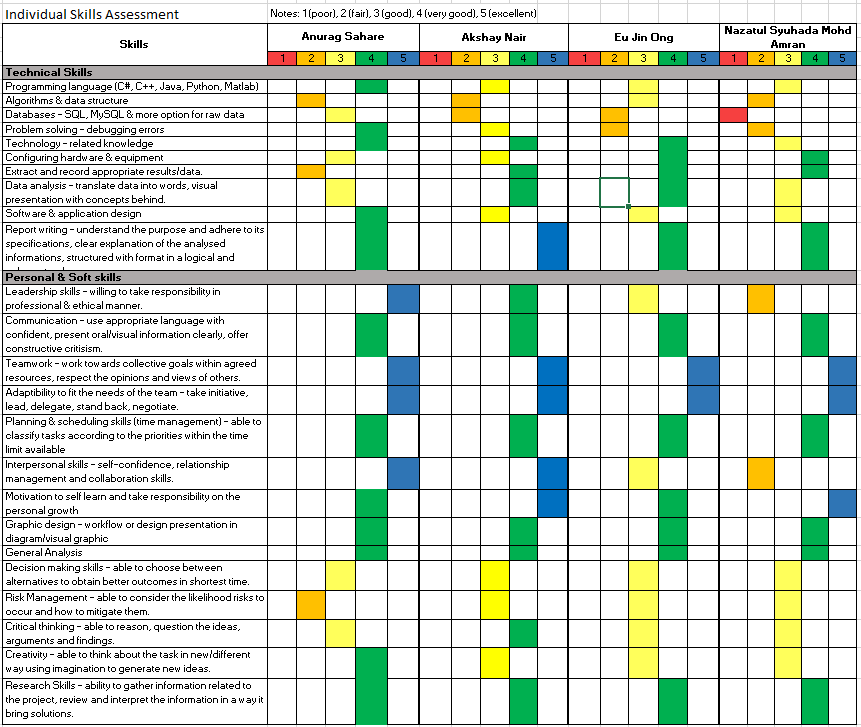
\includegraphics[width=1\linewidth]{images/iusa.png}
    \caption{Individual Skills Assessment}
    \label{fig:team_isa}
\end{figure}

As mentioned earlier. these sections and their tasks were assigned to members based on each of their skills, knowledge and confidence as seen in Figure \ref{fig:team_isa}. The \textit{Individual Skills Assessment} (ISA) was a crucial part of the project to get a better understanding of each team members' skills and how best to assign tasks. Members who were excelled at programming and analytics were assigned more technical responsibilities and so forth. It can be seen in the ISA that the distribution of skills is roughly even throughout the team and so no tasks were restricted to specific members.

\subsection{Meetings and Notes}
As previously mentioned, weekly meetings were held with the group and project supervisors. An example of the weekly task list produced can be seen in Figure \ref{fig:task_list}. These were important to ensure progress was being made, as well as evidencing the progress of the project for both InterDigital and the supervisor.

\begin{figure}[ht]
    \centering
    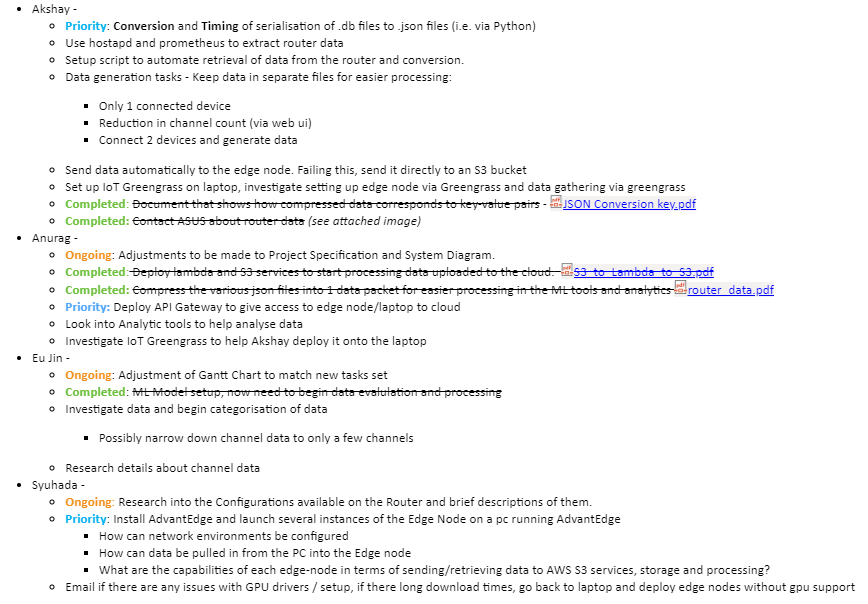
\includegraphics[width=1\linewidth]{images/Task_list.png}
    \caption{Weekly sprint-based list that includes the on-going task, priority and completed tasks assigned for each team members.}
    \label{fig:task_list}
\end{figure}

Meeting minutes were also recorded for every meeting to ensure knowledge and activity in meetings was available for any persons not present in the meeting and also as a record for any changes or developments to not be forgotten. These have all been included within the project archive and can be found within the Project Directory Listing \ref{}.

\subsection{Communication within the Team}
The project team can effectively communicate through the informal weekly meetings or within the formal project meeting with the InterDigital’s lead contact. Information can be shared through anything in the form of written notes to complex extension of files. As part of the responsibility, the project manager has identified the method and approved way of communicating. These includes communication medium shown in Table \ref{tab:communication}. The main focus of these being used as the primary medium is to ensure professionalism within the team and separation from other popular social media platforms so as to ensure responsiveness to any notifications.
\begin{table}[ht]
    \centering
    \begin{tabular}{p{14cm}l}
      \hline
      \textbf{Microsoft Teams}  \\
      \hline 
         \begin{itemize}
             \item Mainly used for online meetings to discuss the progress made, issue encountered and idea for improvement. Make it easier to communicate especially screen can be shared by individual participant.
             \item Information, data or documents can be shared in the folders for everyone in the group to access and download. Any modification can be made online on the documents.
             \item Base for the offline discussion on the general timeline.
         \end{itemize} \\
         \hline
      \textbf{Outlooks (email)}  \\
            \hline 
         \begin{itemize}
             \item The medium used to communicate with the supervisor (university) and the client (company’s representative).
             \item To update and summarize the meetings’ contents, as well as the status report (list of team members’ progress and ongoing tasks).
             \item The reminder for the scheduled meetings.
         \end{itemize} \\
         \hline
    \end{tabular}
    \caption{Communication medium used in the project between the team members, supervisor and InterDigital Partner.}
    \label{tab:communication}
\end{table}

% \section{Technical Planning}
\subsection{Gantt Chart}
\label{gantt_chart}
A Gantt chart was produced to keep track of the progress of the project which can be seen in Appendix \ref{appendix:Gantt}. The chart was produced such that the work done is recorded down on a daily basis with the weekends being excluded. Each completed task is marked with a line, while a dotted line is used for tasks that will be updated as the project progresses. The Gantt chart is split into several sections which includes project preparations, meetings, tasks and submissions. The project preparations section includes the tasks involved before starting off with the group design project. 

The meeting section in the Gantt Chart also shows the meeting schedule, that were held every week. Each meetings held, would concern different individuals depending on the sprint task for that week. 

The next section describes the main tasks carried out and the progress of each task were tracked daily. New tasks were added as the project progresses. The tasks mainly includes router data and transmission where we managed to achieve most of the goals. Next, the goal of extracting, transforming and loading the JSON files into the S3 cloud storage service was achieved. The goal of training the model as well as validating and evaluating the performance was also achieved. The machine learning model developed was able to get deployed onto the edge node set up by IOT Greengrass Core for real time data inference. However, the OTT application for auto-tuning of the router configurations was not developed as discussed in the Conclusions Section \ref{section:Project Setbacks}. The development of the OTT application is included in the future work section. A web application was developed instead which shows the results of the real time data classification including the timings of the classification.

The final section shows the deadline of the required work submission. Each deadline is marked with a red line on the Gantt chart.

\section{Risk Assessment}
Managing risk is one of the main aspects of project management. Future events can often be determined and their positive or negative impacts to the project. Therefore a plan to deal with those impacts can be designed to mitigate the negative impacts as much as possible. The possibility of the risk and contingency plans which are essential to the risk analysis are provided as below in Figure \ref{fig:risk}.

\begin{figure}[ht]
    \centering
    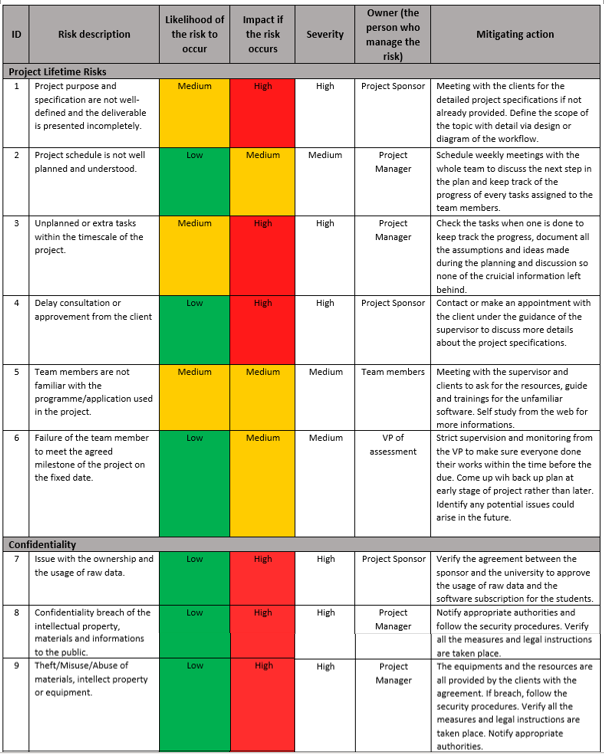
\includegraphics[width=1\textwidth]{images/Risk_1.PNG}
\end{figure}
 
 \begin{figure}[ht]
    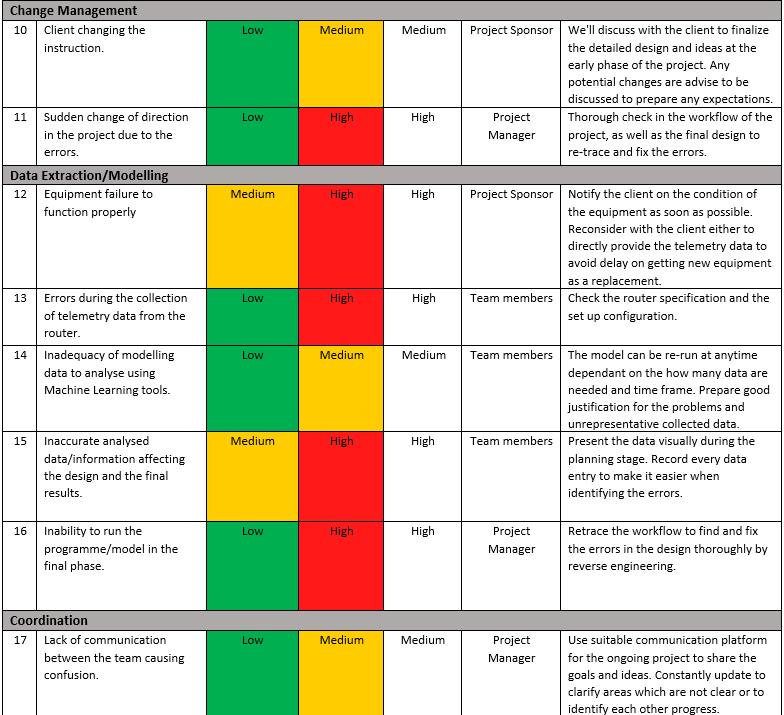
\includegraphics[width=1\textwidth]{images/Risk_2.PNG}
    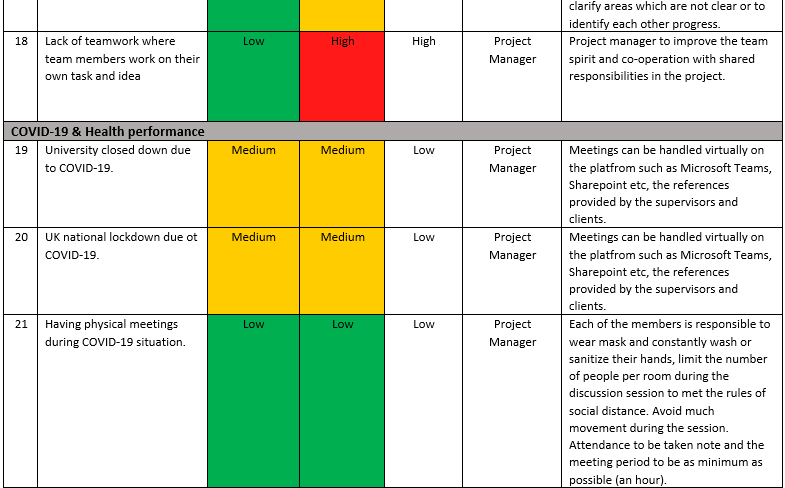
\includegraphics[width=1\textwidth]{images/Risk_3.png}
\end{figure}

 \begin{figure}[t]
    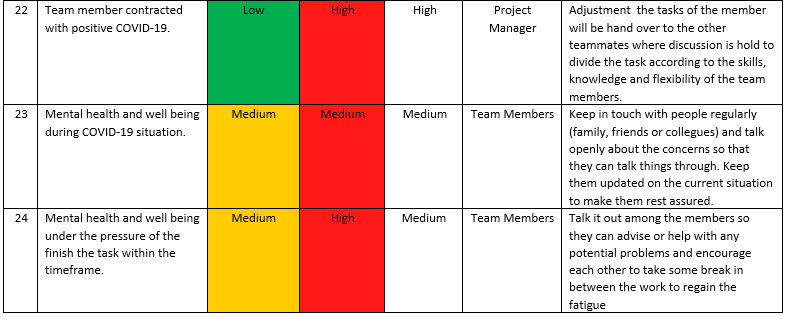
\includegraphics[width=1\textwidth]{images/Risk_4.png}
    \caption{Risk Analysis and Mitigation action.}
    \vspace*{6in}
    \label{fig:risk}
\end{figure}